\documentclass[a4paper,9pt]{extarticle}

\newcommand\hmmax{0}
\newcommand\bmmax{0}

\newlength{\blackoutwidth}
\newcommand{\blackout}[1]
{%necessary comment
  \settowidth{\blackoutwidth}{#1}%necessary comment
  \rule[-0.3em]{\blackoutwidth}{1.125em}%necessary comment
}

\newcommand\cincludegraphics[2][]{\raisebox{-0.2\height}{\includegraphics[#1]{#2}}}
\newcommand\Tstrut{\rule{0pt}{2.1ex}}  
\newcommand\Bstrut{\rule[-0.9ex]{0pt}{0pt}}
\newcommand{\TBstrut}{\Tstrut\Bstrut}

\PassOptionsToPackage{usenames,dvipsnames}{xcolor}
\PassOptionsToPackage{colorlinks,linktoc=all}{hyperref}
\usepackage{balance}       % to better equalize the last page
\usepackage{graphics}      % for EPS, load graphicx instead 
\usepackage[T1]{fontenc}   % for umlauts and other diaeresis
\usepackage{txfonts}
\usepackage{cellspace}
\usepackage{tabularx}
\usepackage{graphicx}
\usepackage{color}
\usepackage{booktabs}
\usepackage{textcomp}
\usepackage{cuted}
\usepackage{capt-of}
\usepackage{enumitem}
\usepackage{multirow}
\usepackage{multicol}
\usepackage[pdflang={en-US},pdftex]{hyperref}


\title{Chemistry HL IA}
\author{Rohan Bansal}
\date{January 2021}

% !TEX root = ../regeneron.tex

% FONTS
%\usepackage[T1]{fontenc}

% Replace default Latin Modern typewriter with its proportional counterpart
% http://www.tug.dk/FontCatalogue/lmoderntypewriterprop/
%\renewcommand*\ttdefault{lmvtt}

%%% OPTION 3 - MTPRO 2 Math + Termes Times + ParaType Sans
\let\myBbbk\Bbbk
\let\Bbbk\relax
\let\bibsep\relax
\let\openbox\relax
\let\proof\relax
\let\endproof\relax
\let\iint\relax
\let\iiint\relax
\let\iiiint\relax
\let\idotsint\relax
%\usepackage{tgtermes}
\usepackage{minted}
\usepackage{amsmath}
\usepackage{blkarray}
% \usepackage[subscriptcorrection,
%             amssymbols,
%             mtpbb,
%             mtpcal,
%             nofontinfo  % suppresses all warnings
%            ]{mtpro2}
% \usepackage{scalefnt,letltxmacro}
% \LetLtxMacro{\oldtextsc}{\textsc}
% \renewcommand{\textsc}[1]{\oldtextsc{\scalefont{1.10}#1}}
% \usepackage[scaled=0.92]{PTSans}

% ICONS
\usepackage{fontawesome}

% CODE

% COLOR
\usepackage[usenames,dvipsnames]{xcolor}
\definecolor{shadecolor}{gray}{0.9}

% SPACING and TEXT
%\usepackage[final,expansion=alltext]{microtype}
%\usepackage[english]{babel}
\usepackage[parfill]{parskip}
\usepackage{afterpage}
\usepackage{framed}
\usepackage{nicefrac}

% EDITING
% line numbering in left margin
\usepackage{lineno}
\renewcommand\linenumberfont{\normalfont
                             \footnotesize
                             \sffamily
                             \color{SkyBlue}}
% ragged paragraphs in right margin
\usepackage{ragged2e}
\DeclareRobustCommand{\sidenote}[1]{\marginpar{
                                    \RaggedRight
                                    \textcolor{Plum}{\textsf{#1}}}}

% Define a paragraph header function
\DeclareRobustCommand{\parhead}[1]{\textbf{#1}~}

% paragraph helper
\DeclareRobustCommand{\PP}{\textcolor{Plum}{\P}~}
\DeclareRobustCommand{\pp}{\textcolor{Plum}{\P}~}

% COUNTERS
\renewcommand{\labelenumi}{\color{black!67}{\arabic{enumi}.}}
\renewcommand{\labelenumii}{{\color{black!67}(\alph{enumii})}}
\renewcommand{\labelitemi}{{\color{black!67}\textbullet}}

% FIGURES
\usepackage{graphicx}
\usepackage[labelfont=bf]{caption}
\usepackage[format=hang]{subcaption}

% TABLES
\usepackage{booktabs}
%\usepackage{dblfloatfix}  % for placing table at bottom of page

% TABLE ALIGNMENT
\usepackage{etoolbox,siunitx}
\robustify\bfseries
\sisetup{detect-weight=true, detect-shape=true, detect-mode=true,
table-format=5.1,
table-number-alignment=center,
separate-uncertainty=true,
input-ignore={,},input-decimal-markers={.}}

% BABEL
% \usepackage{polyglossia}


% ALGORITHMS
\usepackage[algoruled]{algorithm2e}
\usepackage{listings}
\usepackage{fancyvrb}
\fvset{fontsize=\normalsize}

% THEOREMS
\usepackage{amsthm}
\newtheorem{theorem}{Theorem}
% \newtheorem{proposition}[proposition]{Proposition}
\newtheorem{prop}{Proposition}


% TODO
%\usepackage{todo}

% HYPERREF
%\usepackage[colorlinks,linktoc=all]{hyperref}
\usepackage[all]{hypcap}
\hypersetup{citecolor=Violet}
\hypersetup{linkcolor=black}
\hypersetup{urlcolor=MidnightBlue}

% CLEVEREF must come after HYPERREF
\usepackage[capitalize]{cleveref}

% ACRONYMS
\usepackage[acronym,smallcaps,nowarn]{glossaries}
% \makeglossaries

% COLOR DEFINITIONS
\newcommand{\red}[1]{\textcolor{BrickRed}{#1}}
\newcommand{\orange}[1]{\textcolor{BurntOrange}{#1}}
\newcommand{\green}[1]{\textcolor{OliveGreen}{#1}}
\newcommand{\blue}[1]{\textcolor{MidnightBlue}{#1}}
\newcommand{\gray}[1]{\textcolor{black!60}{#1}}

% LISTINGS DEFINTIONS
\usepackage{listings}
\lstdefinestyle{alp_style}{
    commentstyle=\color{OliveGreen},
    numberstyle=\tiny\color{black!60},
    stringstyle=\color{BrickRed},
    basicstyle=\ttfamily\scriptsize,
    breakatwhitespace=false,
    breaklines=true,
    captionpos=b,
    keepspaces=true,
    numbers=none,
    numbersep=5pt,
    showspaces=false,
    showstringspaces=false,
    showtabs=false,
    tabsize=2
}
\lstset{style=alp_style}

\usepackage[margin=.8in,
includehead,
includefoot,]{geometry}

\usepackage{fancyhdr}
\pagestyle{fancy}
\fancyhf{}
\fancyfoot[R]{\thepage}
\renewcommand{\headrulewidth}{0pt}
\renewcommand{\footrulewidth}{0pt}

\usepackage[nottoc,numbib]{tocbibind}


% !TEX root = ../set_recommendation.tex

\DeclareRobustCommand{\mb}[1]{\ensuremath{\boldsymbol{\mathbf{#1}}}}
%\DeclareRobustCommand{\mb}[1]{\mathbold{#1}}

\DeclareRobustCommand{\KL}[2]{\ensuremath{\textrm{KL}\left(#1\;\|\;#2\right)}}

\DeclareMathOperator*{\argmax}{arg\,max}
\DeclareMathOperator*{\argmin}{arg\,min}

\newcommand{\yqm}{y_{qm}}
\newcommand{\xum}{x_{um}}
\newcommand{\xuk}{x_{uk}}
\newcommand{\yuk}{y_{uk}}
\renewcommand{\mid}{~\vert~}
\newcommand{\prm}{\:;\:}

\newcommand{\mbw}{\mb{w}}
\newcommand{\mbW}{\mb{W}}

\newcommand{\mbx}{\mb{x}}
\newcommand{\mbX}{\mb{X}}

\newcommand{\mby}{\mb{y}}
\newcommand{\mbY}{\mb{Y}}

\newcommand{\mbz}{\mb{z}}
\newcommand{\mbZ}{\mb{Z}}

\newcommand{\mbI}{\mb{I}}
\newcommand{\mbone}{\mb{1}}

\newcommand{\mbL}{\mb{L}}

\newcommand{\mbtheta}{\mb{\theta}}
\newcommand{\mbTheta}{\mb{\Theta}}
\newcommand{\mbomega}{\mb{\omega}}
\newcommand{\mbOmega}{\mb{\Omega}}
\newcommand{\mbsigma}{\mb{\sigma}}
\newcommand{\mbSigma}{\mb{\Sigma}}
\newcommand{\mbphi}{\mb{\phi}}
\newcommand{\mbPhi}{\mb{\Phi}}

\newcommand{\mbalpha}{\mb{\alpha}}
\newcommand{\mbbeta}{\mb{\beta}}
\newcommand{\mbgamma}{\mb{\gamma}}
\newcommand{\mbeta}{\mb{\eta}}
\newcommand{\mbmu}{\mb{\mu}}
\newcommand{\mbrho}{\mb{\rho}}
\newcommand{\mblambda}{\mb{\lambda}}
\newcommand{\mbzeta}{\mb{\zeta}}

\newcommand\dif{\mathop{}\!\mathrm{d}}
\newcommand{\diag}{\textrm{diag}}
\newcommand{\supp}{\textrm{supp}}

\newcommand{\E}{\mathbb{E}}
\newcommand{\V}{\mathbb{V}}
\newcommand{\bbH}{\mathbb{H}}

\newcommand{\bbN}{\mathbb{N}}
\newcommand{\bbZ}{\mathbb{Z}}
\newcommand{\bbR}{\mathbb{R}}
\newcommand{\bbS}{\mathbb{S}}

\newcommand{\cL}{\mathcal{L}}
\newcommand{\cS}{\mathcal{S}}
\newcommand{\cD}{\mathcal{D}}

\newcommand{\cN}{\mathcal{N}}
\newcommand{\cT}{\mathcal{T}}

\newcommand{\mult}{\textrm{Mult}}
\newcommand{\dirichlet}{\textrm{Dirichlet}}
\newcommand{\Gam}{\textrm{Gamma}}
\newcommand{\Pois}{\textrm{Poisson}}
% !TEX root = recommending-interesting-writing.tex

\newacronym{ELBO}{elbo}{evidence lower bound}
\newacronym{GMM}{gmm}{Gaussian mixture model}
\newacronym{KL}{kl}{Kullback-Leibler}
\newacronym{LDA}{lda}{latent Dirichlet allocation}
\newacronym{SVI}{svi}{stochastic variational inference}
\newacronym{DEF}{def}{deep exponential family}
\newacronym{rfs}{rfs}{\textsc{rankfromsets}}
\newacronym{bert}{bert}{\textsc{bert}}
\newacronym{NLP}{NLP}{natural language processing}
\newacronym{ctpf}{ctpf}{collaborative topic Poisson factorization}

\usepackage[%
minnames=1,maxnames=99,maxcitenames=2,
style=numeric, %alphabetic, numeric, authoryear
giveninits=true, % true, false
hyperref,
natbib,
backend=biber,
sorting=nyt
]{biblatex}%

% suppress 'in'
\renewbibmacro{in:}{}

\bibliography{bib}
\begin{document}

% !TEX root = ../math_ia.tex
\section{Introduction}
\label{sec:introduction}
I first became intrigued with the concept of moment of inertia when learning about rotating bodies such as flywheels and ferris wheels. I understood that these bodies were "moving" and stored kinetic energy, but they had no linear movement, leaving me somewhat confused about the general premise for calculating their stored energy. I soon realized that an understanding of rotational movement and a particle based approach could higlight the parallels between linear kinetic energy and rotational kinetic energy which led to the discovery of moments of inertias. The literal definition of moment of inertia is the opposition of a body to having its speed of rotation abbout an axis altered by the application of a torque (the rotational equivalent of traditional inertia). It plays a major role in rotational dynamics and has a host of applications when it comes to motors, wheels, and machinery. Its ability to serve as a measure of the resistance to angular motion for a body makes it equally important as traditional inertia, which dictates many physical aspects of our daily lives. Pure rolling motion, bridge building, and flywheels in engines are all predicated on the concept of moment of inertia, and thus the idea becomes exceedingly crucial in the study and implementations of engineering. Scientists and mathematicians are continuing to look for methods to calculate more intricate moments of inertias to improve current physical systems and create new practical technology~\parencite{Young_Freedman_Young_2020}.


This interesting concept lends itself to a a mathematical investigation for deriving moment of inertia formulas for progressively more complex mass distributions. Because of the reliance of moment of inertia on the geometric makeup of a body, I decided to investigate the various approaches that are used to calculate the values and derive some of the most commonly used formulas in modern physics and mathematics. My combined interest in crucial physical applications, such as rotation, as well as the beauty of integration provide a clear motivation for the study and emphasize the personal nature of the investigation.

% !TEX root = ../math_ia.tex
\section{Background}
\label{sec:background}

\subsection{Kinetic Energy and Physics Definitions}
Kinetic energy is a measure of the energy of a moving body. The formula for the calculation of kinetic energy of a body moving with translational velocity $v$ and a mass $M$, with the assumption that the body is rigid and the center of mass is moving at the same constant velocity is shown in \cref{eq:basic_kinetic_energy}~\parencite{Young_Freedman_Young_2020}.

\begin{equation}
KE = \frac{1}{2}Mv^2
\label{eq:basic_kinetic_energy}
\end{equation}

For a complex body defined by a set of particle-masses with unique energies, the principle of superposition can be applied to produce \cref{eq:comb_kinetic_energy} in which the kinetic energies of each particle $i$ are summed.

\begin{equation}
KE = \sum_i\frac{1}{2}M_iv_i^2
\label{eq:comb_kinetic_energy}
\end{equation}

Thus, the calculation of kinetic energy of a rigid body exhibiting translational motion is based solely on mass and velocity and its geometric configuration has no impact on the quantity. However, for rotational motion, this premise can no longer be accepted because each particle has a unique linear velocity depending on its distance from the axis of rotation. Consider a thin disk rotating about a vertical axis that passes perpendicularly through its center as shown in \cref{fig:rotating_disk}.

% !TEX root = ../math_ia.tex
\begin{figure}[H]
  \centering
  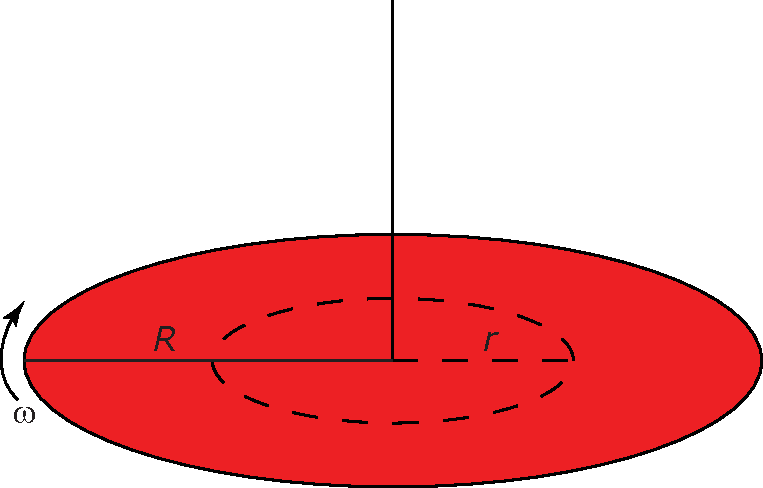
\includegraphics[width=0.35\linewidth]{fig/images/rotating_disk.pdf}
  \caption{A solid disk rotating about a centered, perpendicular axis with a constant angular velocity $\omega$}
  \label{fig:rotating_disk}
\end{figure}

Although each point of the disk is rotating with a constant angular velocity $\omega$, the linear velocity of each point is different. This can be easily determined using an understanding of rotation and time. The entire disk must undergo one complete revolution in time $\frac{2\pi}{\omega}$, but the distance that a point must travel in that time is dependent on its distance from the axis. For a point at a distance of $r$ from this axis, this distance is simply the circumfrence of a circle with radius $r$, or $2\pi r$. Using the formula $speed = \frac{distance}{time}$, the speed of this particle is defined by \cref{eq:v_and_w}. Thus, the rotating disk can actually be thought of as a combination of thin rings each consisting with particles moving at a unique velocity. 

\begin{equation}
v = \frac{2\pi r}{\frac{2\pi}{\omega}} = r\omega
\label{eq:v_and_w}
\end{equation}

For better generalization of this formula in instances where the velocity is not directly perpendicular to the axis of rotation, velocity can also be written as a cross product of the angular velocity vector (in the same direction as the axis of rotation) $\bm{\omega}$ and the position vector of the particle $\bm{r_i}$ as:

\begin{equation}
\bm{v_i} = \bm{\omega} \times \bm{r_i}
\end{equation}
and the angular velocity vector as:

\begin{equation}
\bm{\omega} = \omega \bm{k}
\end{equation}
where $\bm{k}$ is simply a unit vector in the direction of the rotational axis and $\omega$ is the magnitude of the angular velocity. Then, the velocity can simplified to:

\begin{equation}
\bm{v_i} = \omega |k \times \bm{r_i}|
\end{equation}

$|\bm{k} \times \bm{r_i}|$ is equivalent to the perpendicular distance between the point and the axis of rotation, which will be proved later. Using this value, we can utilize the traditional formula for kinetic energy to calculate the energy for a single rotating particle as:

\begin{equation}
R.K.E._i = \frac{1}{2}m_i\omega^2 |\bm{k} \times \bm{r_i}|^2
\label{eq:particle_rotational_energy}
\end{equation}

and the rotational energy for the entire body as:

\begin{equation}
R.K.E. = \sum_i \frac{1}{2}m_i\omega^2 |\bm{k} \times \bm{r_i}|^2
\label{eq:total_rotational_energy}
\end{equation}

To simplify this equation, the moment of inertia of a body is empirically defined as:

\begin{equation}
I = \sum_i m_i|\bm{k} \times \bm{r_i}|^2
\label{eq:total_moment_inertia}
\end{equation}

which for a single particle can be simplified to:

\begin{equation}
I = mr^2
\label{eq:simple_moment_inertia}
\end{equation}

where $r$ is the perpendicular distance from the particle to the axis.

The general formula for rotational kinetic energy can then be defined by \cref{eq:basic_rke} using two values, the rotational velocity $\omega$ and the moment of inertia $I$, which for a body rotating at a constant velocity about a fixed axis are constants (similar to $M$ and $v$ for traditional kinetic energy)~\parencite{Young_Freedman_Young_2020}.

\begin{equation}
R.K.E = \frac{1}{2}I\omega^2
\label{eq:basic_rke}
\end{equation}

Plugging in \cref{eq:simple_moment_inertia} and \cref{eq:v_and_w} to the equation for rotational kinetic energy shows that the final units remain the same as that for traditional kinetic energy presented in \cref{eq:basic_kinetic_energy}. Moment of inertias are also utilized to calculate angular momentum about a point which has many identical properties to traditional momentum, including conservation and collision governance. Using this information, I will derive moment of inertia formulas for a multitude of common bodies in motion.

\subsection{Vector Cross Products}

The formula for moment of inertia relies on the magnitude of a cross product. The general formula for the magnitude of a cross product is defined as~\parencite{Hass_Heil_Weir_2018}:

\begin{equation}
|\bm{u} \times \bm{v}| = |\bm{u}||\bm{v}|\sin{\theta}
\label{eq:cross_product}
\end{equation}

where $\theta$ is the angle between the two vectors.

This can be proved using basic vector rules:

\begin{gather*}
\text{Let } \bm{u} = \begin{bmatrix}u_1\\u_2\\u_3\end{bmatrix} \text{ and } \bm{v} = \begin{bmatrix}v_1\\v_2\\v_3\end{bmatrix} \\
\bm{u} \times \bm{v} = \begin{vmatrix}
\bm{i} & \bm{j} & \bm{j}\\
u_1 & u_2 & u_3 \\
v_1 & v_2 & v_3
\end{vmatrix} = \begin{vmatrix}
u_2 & u_3 \\
v_2 & v_3
\end{vmatrix}\bm{i} - \begin{vmatrix}
u_1 & u_3 \\
v_1 & v_3
\end{vmatrix}\bm{j} + \begin{vmatrix}
u_1 & u_2 \\
v_1 & v_2
\end{vmatrix}\bm{k} = \begin{bmatrix}u_2v_3 - u_3v_2\\u_3v_1 - u_1v_3\\u_1v_2 - u_2v_1\end{bmatrix}\\
\end{gather*}

Then, the squared-magnitude of the cross-product can be defined as:
\begin{align*}
|\bm{u} \times \bm{v}|^2 &= (\bm{u} \times \bm{v}) \cdot (\bm{u} \times \bm{v}) \\
&= (u_2v_3 - u_3v_2)^2 + (u_3v_1 - u_1v_3)^2 + (u_1v_2 - u_2v_1)^2 \\
&= u_2^2v_3^2 + u_3^2v_2^2 + u_1^2v_3^2 + u_3^2v_1^2 + u_1^2v_2^2 + u_2^2v_1^2 - 2(u_2u_3v_2v_3 + u_1u_3v_1v_3 + u_1u_2v_1v_2)
\end{align*}

We can also observe two other intriguing results:
\begin{align*}
(\bm{u} \cdot \bm{v})^2 &= (u_1v_1 + u_2v_2 + u_3v_3)^2 \\
&= u_1^2v_1^2 + u_2^2v_2^2 + u_3^2v_3^2 + 2(u_2u_3v_2v_3 + u_1u_3v_1v_3 + u_1u_2v_1v_2) \\
\end{align*}
\begin{align*}
(|\bm{u}||\bm{v}|)^2 &= (\sqrt{u_1^2 + u_2^2 + u_3^2}\sqrt{v_1^2 + v_2^2 + v_3^2})^2 \\
&= (u_1^2 + u_2^2 + u_3^2)(v_1^2 + v_2^2 + v_3^2) \\
&= u_2^2v_3^2 + u_3^2v_2^2 + u_1^2v_3^2 + u_3^2v_1^2 + u_1^2v_2^2 + u_2^2v_1^2 + u_1^2v_1^2 + u_2^2v_2^2 + u_3^2v_3^2
\end{align*}

By subtracting the second result from the third result, we can acquire the first result, leading to the formula:
\begin{align*}
|\bm{u} \times \bm{v}|^2 &= (|\bm{u}||\bm{v}|)^2 - (\bm{u} \cdot \bm{v})^2 \\
&= (|\bm{u}||\bm{v}|)^2 - (|\bm{u}||\bm{v}|\cos{\theta})^2 \\
&= (|\bm{u}||\bm{v}|)^2 - (|\bm{u}||\bm{v}|)^2\cos^2{\theta} \\
&= (|\bm{u}||\bm{v}|)^2(1 - \cos^2{\theta}) \\
&= (|\bm{u}||\bm{v}|)^2\sin^2{\theta}
\end{align*}

This result can then be square rooted, resulting in the initial theorem presented in \cref{eq:cross_product}. Because of this formula, the cross product between a unit vector and the position vector can also represent the perpendicular distance between the direction of the unit vector and the specific position. This premise is adopted for this investigation.

\subsection{Parallel Axis Theorem}

To calculate the moment of inertia for more complex bodies, the parallel axis theorem is often utilized to relate the moment of inertia about an axis passing through the center of mass of a body to a parallel axis at a distance $d$ from the central axis~\parencite{Abdulghany_2017}. \cref{eq:parallel_axis_formula} describes the theorem, where $I_{cm}$ is the moment of inertia through an axis passing through the center of mass, $M$ is the mass of the body, and $I'$ is the resultant moment of inertia through the parallel axis. This equation is applicable for any body, regardless of shape or dimensions.

\begin{equation}
I' = I_{cm} + Md^2
\label{eq:parallel_axis_formula}
\end{equation}

To prove this relationship, consider a lamina with mass $M$ located in the $X-Y$ plane whose center of mass is located at the origin as in \cref{fig:parallel_axis_lamina}. A general point $i$ is depicted and has coordinated $(x_i, y_i)$ and the parallel axis passes through $O$ which has coordinates $(a, b)$.

% !TEX root = ../math_ia.tex
\begin{figure}[H]
  \centering
  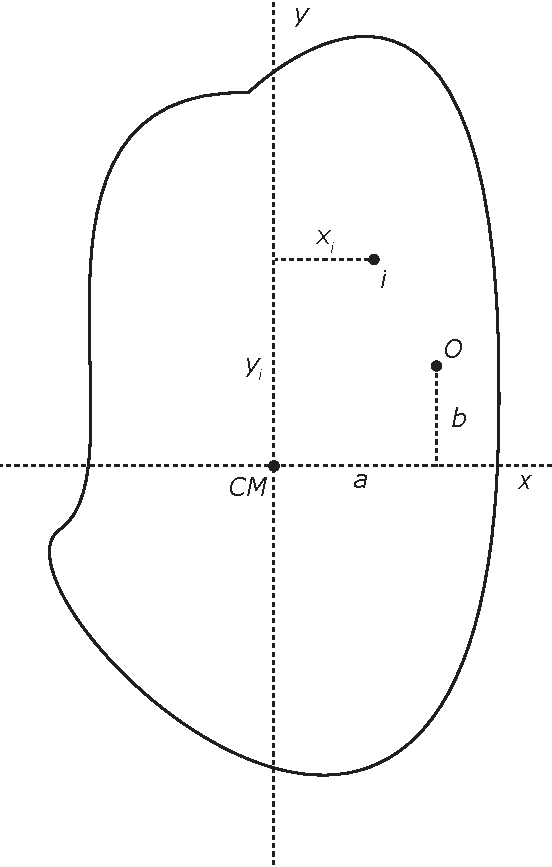
\includegraphics[width=0.25\linewidth]{fig/images/parallel_axis_lamina.pdf}
  \caption{A plain lamina in the $X-Y$ plane with its center of mass located at the origin}
  \label{fig:parallel_axis_lamina}
\end{figure} 

Because the center of mass is simply a weighted average of the mass of individual points on the lamina and the center of mass coincides with the origin, we can deduce:

\[x_{CM} = \frac{\sum_i m_ix_i}{M} = 0 \]
\[y_{CM} = \frac{\sum_i m_iy_i}{M} = 0 \]

Using the definition of moment of inertia for a particle and denoting the distance between point $i$ and point $O$ as $r_{iO}$, we can see $I_O = \sum_i m_i r_{iO}^2$. Using the distance formula, we have:

\[r_{iO}^2 = (x_i-a)^2 + (y_i-b)^2\]

Then,

\begin{align*}
I_O &= \sum_i m_i r_{iO}^2 \\
&= \sum_i m_i \left[(x_i-a)^2 + (y_i-b)^2\right] \\
&= \sum_i m_i \left[x_i^2 + a^2 - 2x_ia + y_i^2 + b^2 - 2y_ib\right]
\end{align*}

Now, using the deductions from the center of mass, the $2x_ia$ and $2y_ib$ terms can be removed, as $\frac{\sum_i m_ix_i}{M} = 0$ and $\frac{\sum_i m_iy_i}{M} = 0$, leaving:

\[I_O = \sum_i m_i (x_i^2 + y_i^2) + \sum_i m_i (a^2 + b^2) \]

Again, the distance formula (and the fact that the center of mass is located at the origin), allows us to see that $(x_i^2 + y_i^2)$ is simply equal to the square of the distance from point $i$ to the origin, or $r_i^2$, and $(a^2 + b^2)$ is equivalent to the square of the distance between point $O$ and the origin, or $d^2$. Then, we have:

\[I_O = \sum_i m_i r_i^2\ + \sum_i m_id^2\]

As we know that the first summation is equivalent to the moment of inertia about the center of mass (the origin) using \cref{eq:total_moment_inertia,eq:simple_moment_inertia}, and $d^2$ is constant, this simplifies to:

\[I_O = I_{CM} + Md^2\]

leaving the initial theorem as presented in \cref{eq:parallel_axis_formula}.


% !TEX root = ../chem_ia.tex
\section{Hypothesis}

\textbf{Increasing the temperature of the reaction between iodine solution and acetone in the presence of hydrocholoric acid catalyst will directly increase the rate of the reaction.}

As discussed earlier, the increase in temperature with the addition of a catalyst allows for a larger proportion of molecules to have sufficient energy greater than the activation energy and induces more frequent successful collisions, resulting in a quicker rate~\parencite{general_catalysts}. The exact activation energy will be determined by the experiment and the hypothesis can then simultaneously be confirmed or rejected.



% !TEX root = ../chem_ia.tex
\section{Variables}

\subsection{Rate Law Experiment}

\textbf{Independent Variable: Concentration of reactants ($\frac{mol}{dm^3}$)} 

It has empirically been confirmed that the rate of a reaction is solely dependent on the rate constant (which is constant at a fixed temperature) and the concentrations of the reactants (and catalysts in the case of specific mechanisms). Thus, to find the rate law for this specific iodination of acetone reaction, a baseline was provided through the initial configuration and then each set of trials manipulated the concentration of a certain reactant ($HCl$, $Acetone$, or $I_2$) for the purpose of comparison. This allowed for the determination of the order of each reactant in the rate law through simple proportions. To make this process easy, the baseline configuration used $5$ $mL$ of each reactant/catalyst, and the manipulated trials doubled these volumes for each reactant to $10$ $mL$. The total volume was held constant through the addition of water, so this doubling in volume of the reactant meant a direct doubling of that reactant's concentration, and thus the effect on the rate could easily be identified. As the rate law is crucial to the determination of the activation energy in the second part of this investigation, the choice of independent variable is justified.

\textbf{Dependent Variable: Time taken for solution to lose its color ($s$)} 

By using the time for the completion of the reaction (once the iodine color has disappeared) and the initial concentration of iodine, the rate of the reaction can be determined for each chosen configuration of reactants. These rates can then be compared to the baseline provided by the initial configuration for the experiment to identify how the changing of concentrations of each reactant impacts the overall rate. By doing this for each reactant, the rate law for the total reaction can be empirically confirmed/found, allowing us to determine the rate constant in the activation energy experiment. Additionally, as time is also the dependent variable for the activation energy experiment, the trials for the first configuration can then be utilized further. Thus, the time taken for the reaction to lose its color is relevant to the overall investigation.

\textbf{Unique Control Variable: Temperature ($K$)} 

Because the temperature impacts the rate constant ($k$), it was crucial to maintain a constant temperature for the determination of the rate formula. As the premise of finding the rate law relies on the resultant rate proportions of changing concentrations, a change in $k$ would introduce a confounding variable and render the results inconclusive. A room temperature of $294.8$ $K$ was taken as this constant temperature for all trials conducted as part of the rate law experiment and it was ensured that all reactants were at this fixed temperature prior to the initialization of the reaction through constant temperature checks via thermometer.

\subsection{Activation Energy Experiment}

\textbf{Independent Variable: Temperature ($K$)} 

As mentioned in the background, the rate constant varies depending on temperature, and the calculation of multiple rate constants at known temperatures can be used to find the activation energy through the Arrhenius equation. The linear relationship between the inverse of the temperature and the natural logarithm of the rate constant allows for simple graphing and gradient calculation which can then be used to find the activation energy, indicating the relevance to the investigation. Because specific temperatures are not required and instead a variety of temperatures are crucial, temperatures in the ranges of $283-285$, $293-298$ (room temperature in the above experiment), $303-308$, and $313-318$ $K$ were used to conduct trials and were manipulated through the use of heated or ice-filled water baths. I refrained from adding higher temperatures for fear of partial evaporation of the reactants, as this would impact concentrations, and lead to erroneous calculations with regards to the rate of reaction and rate constant.

\textbf{Dependent Variable: Time taken for solution to lose its color ($s$)} 

This is an easily observable characteristic of the reaction which allows for the determination of the completion of the reaction and thus leads to a straightforward process for quantifying the rate of the reaction (as discussed previously). All times were calculated in seconds ($s$) for consistency and to maintain the appropriate rates for $k$ for a second order reaction ($\frac{dm^3}{mol \cdot s}$). Because the rate constant can then be used to determine the activation energy of the reaction, this choice of a dependent variable is entirely relevant to the investigation and allows for the answering of the initial research question. 

\textbf{Unique Control Variable: Volumes of reactants ($cm^3$)} 

All trials utilized for this experiment had identical volumes of each reactant and identical total volumes leading to the same concentration of each reactant for all trials. These volumes were chosen to make iodine the limiting reactant and provide large excess of $HCl$ and $Acetone$, so as to ensure that all iodine was used up after the reactions completion and prevent large fluctuations in the concentration of the other reactants which could also impact the rate. This was necessary as the experiment was designed to investigate the change of the rate due to temperature alone, and thus the control variable was necessary.

\subsection{Universal Controls}

\textbf{Pressure}

Large fluctuations in pressure can impact the rate of evaporation of the reactants involved in the experiment which would affect the concentrations and induce erroneous rate calculations. Pressure changes have also been found to impact the kinetics of molecules with regards to aqueous reactants which could have introducing confounding causes for the change in the rate constant with varying temperatures. To control for pressure, all experiments were carried out in a controlled environment and a uniform laboratory at a fixed altitude. 

\textbf{Purity/Molarity of Reactants}

As the molarity of the reactants was used to determine their respective concentrations, it was crucial that these molarities were accurately measured and maintained for the duration of all trials. To control, all reactants were properly diluted prior to the beginning of the experiment and sufficient quantities were produced so as to allow for consistent utilization for all trials. The diluted solutions were stored safely to prevent any external contamination or evaporation.

\textbf{Physical Manipulation of Reaction}

Swirling of the reaction mixture is crucial for ensuring that the reactants evenly mix throughout and helps faciliate more frequent collisisons between particles (thereby increasing the rate of the reaction). To ensure that discrepancies in swirling did not account for the various results, all trials were given $30$ seconds of swiriling and then allowed to sit to completion. This attempted to control the confounding variable and let the reaction occur naturally after all reactants were adequately mixed.


% !TEX root = ../chem_ia.tex
\section{Methodology}

\subsection{Apparatus}

\begin{table}[h!]
\centering

\begin{tabular}{m{5cm} m{5cm} m{4cm}} 
 \toprule
 Chemicals & Glassware & Miscellaneous \\
 \midrule
	\begin{itemize}[]
	  \item $120$ $cm^3$ $1 M$ $HCl$
	  \item $120$ $cm^3$ $4 M$ $Acetone$
	  \item $120$ $cm^3$ $.005 M$ $I_2$ solution 
	  \item $165$ $cm^3$ Distilled $H_2O$
	\end{itemize} & 
	\begin{itemize}[]
	  \item $100$ $mL$ Erlenmeyer Flask
	  \item $1000$ $mL$ Beaker
	  \item $10$ $mL$ Graduated Cylinder
	  \item Test Tube(s)
	\end{itemize} & 
	\begin{itemize}[]
	  \item Ice
	  \item Thermometer
	  \item Ring Stand
	  \item Poly Water Bath
	  \item $2x$ Beaker Clamp
	  \item Water Source
	\end{itemize} \\
  \bottomrule
\end{tabular}
\caption{Materials}
\label{table:apparatus}
\end{table}

\subsection{Experimental Procedure}
\subsubsection{Rate Law Determination}
	\begin{enumerate}[itemsep=-1ex]
	  \item Prepare a water bath at room temperature in a $1000$ $mL$ beaker.
	  \item Clamp a $100$ $mL$ erlenmeyer flask and a separate test tube into the water bath.
	  \item Measure out the appropriate amounts of $HCl$, $Acetone$, and $H_2O$ (as listed in \cref{table:1_config}) into the $10$ $mL$ graduated cylinder and add these substances to the clamped erlenmeyer flask.
	  \item Measure out the appropriate amount of $I_2$ (as listed in \cref{table:1_config}) into the $10$ $mL$ graduated cylinder and pour into the clamped test tube.
	  \item Ensure that the the reactants in the test tube and flask are fully immersed in the water bath and allow 5 minutes for temperature equilibrium to be reached.
	  \item Record the water bath temperature after this period is complete. Attempt to maintain this temperature for all trials to limit potential confounding results for rate law determination.
	  \item Remove the test tube containing the iodine solution and immediately add its contents to the flask containing $HCl$, $Acetone$, and $H_2O$, starting a timer after the addition.
	  \item Swirl the reaction mixture by gently swirling the ring for $30$ $s$ and then allow the solution to sit.
	  \item When the iodine color (brownish-red) has completely disappeared, stop the timer and record the total reaction time (as the reaction is complete).
	  \item Clean the glassware thoroughly and dry (it is not necessary to clean the test tube as it will always contain iodine solution with a constant concentration).
	  \item Repeat steps 2-10 two more times for configuration $\#1$ in \cref{table:1_config}.
	  \item Repeat steps 2-11 for all remaining configurations in \cref{table:1_config}.
	  \item Thoroughly clean all glassware and dispose of any leftover products/substances safely.
	\end{enumerate}

\subsubsection{Activation Energy Determination}
	\begin{enumerate}[itemsep=-1ex]
	  \item Prepare a water bath at temperature within the range listed in \cref{table:2_config} either in the Pro Water Bath (for high temperatures) or in a $1000$ $mL$ beaker with ice (for the low temperature).
	  \item Clamp a $100$ $mL$ erlenmeyer flask and a separate test tube into the water bath.
	  \item Measure out the appropriate amounts of $HCl$, $Acetone$, and $H_2O$ (as listed in \cref{table:2_config}) into the $10$ $mL$ graduated cylinder and add these substances to the clamped erlenmeyer flask.
	  \item Measure out the appropriate amount of $I_2$ (as listed in \cref{table:2_config}) into the $10$ $mL$ graduated cylinder and pour into the clamped test tube.
	  \item Extra care should be taken to measure out exact volumes of the reactants, as they must be controlled for accurate determination of temperature-dependence on the rate constant.
	  \item Ensure that the the reactants in the test tube and flask are fully immersed in the water bath and allow 5 minutes for temperature equilibrium to be reached.
	  \item Record the water bath temperature after this period is complete.
	  \item Remove the test tube containing the iodine solution and immediately add its contents to the flask containing $HCl$, $Acetone$, and $H_2O$, starting a timer after the addition.
	  \item Swirl the reaction mixture by gently swirling the ring for $30$ $s$ and then allow the solution to sit.
	  \item When the iodine color (brownish-red) has completely disappeared, stop the timer and record the total reaction time (as the reaction is complete).
	  \item Clean the glassware thoroughly and dry (it is not necessary to clean the test tube as it will always contain iodine solution with a constant concentration).
	  \item Repeat steps 2-11 two more times for temperature $\#1$ in \cref{table:2_config}.
	  \item Repeat steps 2-12 for all remaining temperature ranges in \cref{table:2_config}.
	  \item Thoroughly clean all glassware and dispose of any leftover products/substances safely.
	\end{enumerate}

\begin{table}[!htb]
    \begin{minipage}{.5\linewidth}
      \caption{Rate Law Experiment}
      \centering
		\begin{tabular}{|c|c|c|c|c|} 
		 \hline
		 \multicolumn{5}{|c|}{Volumes $(mL)$} \\
		 \hline
		$HCl$ & $Acetone$ & $I_2$ & $H_2O$ & Total \\
		  \hline
		  $5$ & $5$ & $5$ & $10$ & $25$ \\
		  \hline
		  $5$ & $5$ & $10$ & $5$ & $25$ \\
		  \hline
		  $5$ & $10$ & $5$ & $5$ & $25$ \\
		  \hline
		  $10$ & $5$ & $5$ & $5$ & $25$ \\
		  \hline
		\end{tabular}
		\label{table:1_config}
    \end{minipage}%
    \begin{minipage}{.5\linewidth}
      \centering
        \caption{Activation Energy Experiment}
		\begin{tabular}{|c|c|c|c|c|c|} 
		 \hline
		  \multirow{2}{*}{Temperature $(\degree C)$} & \multicolumn{5}{c|}{Volumes $(mL)$} \\
		  	\cline{2-6}
		 	& $HCl$ & $Acetone$ & $I_2$ & $H_2O$ & Total \\
		  \hline
		  $10-15$ & $5$ & $5$ & $5$ & $10$ & $25$ \\
		  \hline
		  $30-35$ & $5$ & $5$ & $10$ & $5$ & $25$ \\
		  \hline
		  $40-45$ & $5$ & $10$ & $5$ & $5$ & $25$ \\
		  \hline
		\end{tabular}
		\label{table:2_config}
    \end{minipage}
    \caption{Experimental Configurations}
    \label{table:config}
\end{table}

\subsection{Risk Assessment}

\begin{enumerate}[label=(\alph*),itemsep=-1ex]
	\item \textbf{Experimental Safety}
		\begin{enumerate}[label=(\roman*)]
			\item Acetone is highly flammable and can cause moderate irritation on repeated exposure to skin. Hydrochloric acid is corrosive and can lead to severe damage to both the eyes and skin in the case of direct contact. Strong iodine solution is partially corrosive and can cause blistering or necrosis of the skin on direct contact~\parencite{acetone, acid, iodoacetone}. To counteract these potential concerns, an apron and goggles were worn for the duration of the experiment. All materials were kept at a moderate distance from the body and spills were immediately cleaned.
			\item Glassware is relatively fragile and any potential breakage can be harmful to those in the lab, both through glass shards and substance spillage. To remedy, extreme caution is used at all times in the lab, especially when handling glassware. In the case that glass did break, the teacher would immediately assist in disposing of any pieces prior to the resumption of the experiment. 
			\item Hot water or glassware can cause sudden reactions and burns of the skin. As water was heated and glassware (with various chemicals) were placed in the water baths, tongs were used at all times to handle warm glass. The water was never directly touched and the water bath was kept closed when not in use.
		\end{enumerate}
	\item \textbf{Environmental Concerns}
	\begin{itemize}[label={}]
	  \item All materials were properly stored and disposed of based on lab best practices and teacher advice to prevent any potential environmental contamination. No limited resources were used nor were any harmful byproducts produced.
	\end{itemize}
	\item \textbf{Ethical Concerns}
	\begin{itemize}[label={}]
	  \item Materials were measured out in small quantities to minimize the potential wastage of any chemicals. No live organisms were employed, so limited ethical concerns were present.
	\end{itemize}
\end{enumerate}

% !TEX root = ../chem_ia.tex
\begin{figure}[!htb]
    \centering
    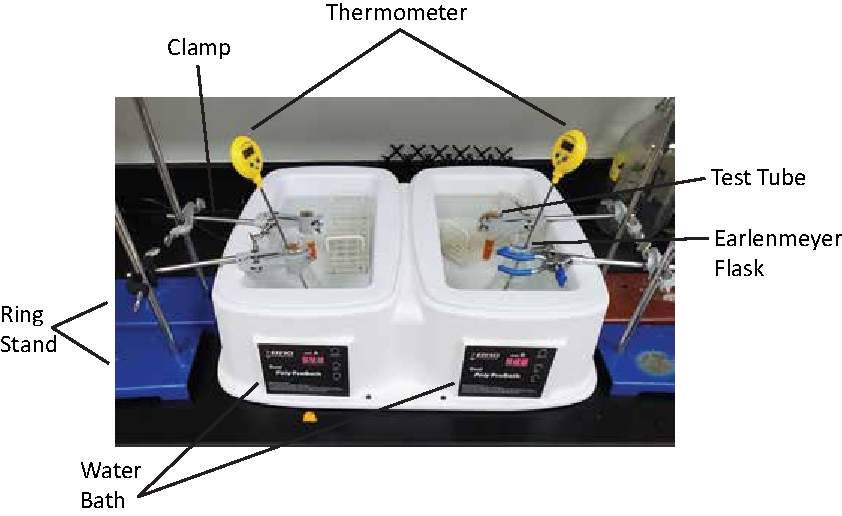
\includegraphics[width=.8\textwidth]{fig/images/visual_setup.pdf}
    \caption{Labelled image depicting the visual setup of the experiment being conducted for two different temperatures.}
    \label{fig:visual_setup}
\end{figure}

% !TEX root = ../chem_ia.tex
\section{Results}

\subsection{Raw Data}

\begin{table}[!htb]
\begin{minipage}[t]{.65\linewidth}
	\centering
	\begin{tabular}{|c|c|c|c|c|c|c|c|c|} 
		 \hline
		 \multirow{2}{*}{Setup} & \multicolumn{5}{c|}{Volumes $(\pm .05 mL)$} & \multicolumn{3}{c|}{Time $(\pm .05 s)$}\\
		 \cline{2-9}
		 & $HCl$ & $Acetone$ & $I_2$ & $H_2O$ & Total & $\#1$ & $\#2$ & $\#3$ \\
		  \hline
		 $\#1$ & $5$ & $5$ & $5$ & $10$ & $25$ & $342$ & $354$ & $331$\\
		  \hline
		  $\#2$ & $5$ & $5$ & $10$ & $5$ & $25$ & $621$ & $682$ & $634$\\
		  \hline
		  $\#3$ & $5$ & $10$ & $5$ & $5$ & $25$ & $161$ & $183$ & $164$\\
		  \hline
		  $\#4$ & $10$ & $5$ & $5$ & $5$ & $25$ & $152$ & $165$ & $153$\\
		  \hline
		\end{tabular}
		\caption{Rate Law Experiment (all trials performed at $294.8$ $K$)}
	\label{table:rate_law_raw_data}
    \end{minipage}%
\begin{minipage}[t]{.35\linewidth}
\centering
	\begin{tabular}{|c|c|c|c|} 
		 \hline
		 Temperature & \multicolumn{3}{c|}{Time $(\pm .05 s)$}\\
		 \cline{2-4}
		 $(\pm .05 K)$ & $\#1$ & $\#2$ & $\#3$ \\
		  \hline
		  $287.1$ & $734$ & $725$ & $756$\\
		  \hline
		  $294.8$ & $342$ & $354$ & $331$\\
		  \hline
		  $306.8$ & $134$ & $142$ & $115$\\
		  \hline
		  $317.5$ & $37$ & $42$ & $46$\\
		  \hline
		\end{tabular}
	\caption{Activation Energy Experiment (all trials carried out with volume setup $\#1$ in \cref{table:rate_law_raw_data})}
	\label{table:activation_energy_raw_data}
	\end{minipage}%
	\caption{Raw Data}
    \label{table:raw_data}
\end{table}

\subsection{Qualitative Data}
\begin{itemize}[]
	  \item The iodine solution had a distinctive brownish-red color, similar to that of rust on iron metal.
	  \item A noticeable loss in color could be observed within the first $30$ seconds of the reaction, even for trials that took over $10$ minutes to come to full completion.
	  \item No observable immediate signs of a vigorous reaction could be observed (outside of the color loss) immediately after the addition of bromine to the remainder of the reactants.
	  \item The acetone had a relatively pungent odor similar to that of nail polish remover.
	  \item The iodine solution seemed to be particularly viscous, especially as opposed to the remainder of the reactants.
	\end{itemize}

\subsection{Calculations}

\subsubsection{Rate Law Experiment}

\begin{table}[h!]
\centering

\begin{tabularx}{\textwidth}{|X|X|}
\hline 
 Rationale & Sample Calculation\\
 \hline
	Firstly, for each volumetric configuration, we must calculate the average time for the three unique trials performed, using the simple arithmetic mean formula:
	\[\bar{t}={\frac {1}{n}}\sum _{i=1}^{n}t_{i}\]
	where $n$ represents the number of trials ($3$).	
	& 
	Example for Setup $\# 1$: \newline

	{$\!\begin{aligned}
	\bar{t} &= \frac{(342 \pm .05) + (354 \pm .05) + (331 \pm .05)}{3} \\
	&= \frac{(1027 \pm .15)}{3} \\
	&= \SI{342 \pm .05}{\second}
	\end{aligned}$} \\
  \hline
Then, we must calculate the concentrations of each reactant based on the total volume and their specific volume using the mole-constant dilution formula:

\[M_1V_1 = M_2V_2 \textit{ or } M_2 = \frac{M_1V_1}{V_2} \]

where $M_1$ is the initial molarity of the reactant, $V_1$ is the initial volume of the reactant, and $V_2$ is the total volume ($25 mL$). We can additionally calculate potential discrepancies for the largest percent uncertainty and then propagate this error for the remaining results.
	& 
	Example for Setup $\# 1$: \newline

	{$\!\begin{aligned}
	\left[I_2\right] &= \frac{\SI{.005}{\molar} \times \SI{5 \pm .05}{\milli\liter}}{\SI{25 \pm .2}{\milli\liter}} = \frac{(.025 + .00025)}{(25 \pm .2)} \\
	&= \frac{(.025 + 1\%)}{(25 \pm .8\%)} = .001 \pm 1.8\% \\
	&= \SI{.001 \pm .000018}{\molar} 
	\end{aligned}$} 

Through an identical process, the final concentrations of $[HCl]$ and $[Acetone]$ can also be determined. Because $[I_2]$ has the smallest quantity, it has the largest percent error of $1.8\%$, which is carried over for all final concentrations. \\
\hline

Using the two above steps, we can then determine the rate for each individual configuration using the previously discussed equation:

\[rate = \frac{[I_2]}{\bar{t}}\]

The same propagation approach is utilized, but the uncertainties are largely irrelevant for the purpose of rate calculation which is predicated on approximation already.
&
Example for Setup $\# 1$: \newline

	{$\!\begin{aligned}
	rate &= \frac{\SI{.001 \pm .000018}{\molar}}{\SI{342 \pm .05}{\second}} \\
	&= \frac{.001 \pm 1.8\%}{342 \pm .01\%} = \num{2.92e-6} \pm 1.81\% \\
	&= \SI{2.92e-6}{\molar\per\second}
	\end{aligned}$} \\

  \hline
After determining the rates for all trials, we can compare the rates for configurations $2-4$ to the baseline provided by $1$ to determine the rate law. As in each of the last $3$ trials, the concentration of one reactant was changed while maintaining the total volume, the concentration of that reactant is doubled for that specific trial. Thus, we can calculate our order $m$ by the formula:

\[m = \log_2 \left(\frac{rate_i}{rate_1}\right)\]

where $rate_i$ is the rate for the given setup and $rate_1$ is the rate for configuration $\#1$. The result must be approximated, as $m$ must be a whole integer $>=0$.
&
Example for Setup $\# 4$ (compared to the baseline of Setup $\# 1$):

	\[m = \log_2 \left(\frac{\num{6.37e-6}}{\num{2.92e-6}}\right) = \log_2 2.18 = 1.12 \approx \bm{1}\]

Thus, the concentration of $HCl$ is first order with respect to the overall reaction based on this determination. The remaining orders are also calculated in the same manner. \\

\hline

\end{tabularx}
\caption{Rate Law Calculations}
\label{table:rate_law_calculations}
\end{table}

Using this process for all trials, the order of $HCl$, $Acetone$, and $I_2$ are found to be $1$, $1$, and $0$ respectively. This confirms the theorized rate law of $rate = k[HCl][CH_3COCH_3]$ and is further supported by the published literature on this subject~\parencite{main_literature}. Through this knowledge, we can now determine the activation energy.
\newpage

\subsubsection{Activation Energy Experiment}

\begin{table}[h!]
\centering

\begin{tabularx}{\textwidth}{|X|X|}
\hline 
 Rationale & Sample Calculation\\
 \hline
 \multicolumn{2}{|>{\hsize=\dimexpr2\hsize+2\tabcolsep+\arrayrulewidth\relax}X|}{The first three steps--calculating the average (mean) time for each temperature, determining diluted concentrations, and finding the rate using those two values--are identical for this section as well, and are thus not included to limit redundancy. \newline}
\\
\hline
After these three steps, we must determine the value of the rate constant $k$, which we can do by utilizing the rate law. As $rate = k[HCl][Acetone]$, we can rearrange to get:

\[k = \frac{rate}{[HCl][Acetone]}\]

Furthermore, the concentrations of $HCl$ and $Acetone$ are consistent for all temperatures as identical volumes were chosen to ease calculations and limit confounding variables.
&
Example for $\SI{294.8}{\kelvin}$: \newline

{$\!\begin{aligned}
	k &= \frac{(\num{2.92e-6} \pm 1.9\%)}{(.2 \pm 1.8\%) \times (.8 \pm 1.8\%)} \\
	&= \num{1.83e-5} \pm 5.5\% \\
	&= \SI{1.83\pm.10e-5}{\cubic\deci\metre\per\mol\per\second}
	\end{aligned}$}
\\
 \hline
 After determining $k$ at each temperature, we will create an Arrhenius graph to determine the activation energy. Taking the natural logarithm of the Arrhenius equation results in:

\[\ln{k} = \left(\frac{-E_a}{R}\right)\frac{1}{T} + \ln{A}\]

Thus, a linear relationship exists between $\ln{k}$ and $\frac{1}{T}$, so these values must be determined (along with their uncertainties) for the purpose of graphing.

&
Example for $\SI{294.8}{\kelvin}$: \newline

{$\!\begin{aligned}
	\frac{1}{T} &= \frac{1}{\SI{294.8 \pm .05}{\kelvin}} = \frac{1}{(294.8 \pm .017\%)} \\
	&=  .00339 \pm .017\% = \SI{3.39\pm.00058e-3}{\per\kelvin}
	\end{aligned}$} 

\rule{0pt}{3ex}   

{$\!\begin{aligned}
	\ln{k} &= \ln{\left(\num{1.83\pm.10e-5}\right)} = \ln{\left(\num{1.83e-5}\right)} + \frac{.10}{1.83} \\
	&= -10.91 \pm .05
	\end{aligned}$} \\

\hline
\end{tabularx}
\caption{Activation Energy Calculations}
\label{table:activation_energy_calculations}
\end{table}

This process is again carried out for all four temperatures, providing the necessary values for graphing purposes.

\subsection{Processed Data}

\begin{table}[!htb]
\begin{minipage}[t]{.5\linewidth}
	\centering
	\begin{tabular}{|c|c|c|c|} 
		 \hline
		 Setup & Avg. Time ($\pm \SI{.5}{\second}$) & Rate ($\si{\molar\per\second}$) \\
		 \hline
		  $\#1$ & $342$ & $\num{2.92\pm.053e-6}$\\
		  \hline
		  $\#2$ & $646$ & $\num{3.10\pm.056e-6}$\\
		  \hline
		  $\#3$ & $169$ & $\num{5.92\pm.107e-6}$\\
		  \hline
		  $\#4$ & $157$ & $\num{6.37\pm.115e-6}$ \\
		  \hline
		 \end{tabular}
		\caption{Rate Law Experiment (all trials performed at $\SI{294.8}{\kelvin}$)}
	\label{table:rate_law_processed_data}
    \end{minipage}%
\begin{minipage}[t]{.5\linewidth}
\centering
	\begin{tabular}{|c|c|c|c|} 
		 \hline
		 Temperature & $k$ ($\si{\cubic\deci\metre\per\mol\per\second}$) & $\frac{1}{T}$ ($\pm .17\%$) ($\si{\per\kelvin}$) & $\ln{k}$ ($\pm .055$) \\
		  \hline
		  $287.1$ & $\num{8.47\pm.47e-6}$ & $\num{3.48e-3}$ & $-11.68$ \\
		  \hline
		  $294.8$ & $\num{1.83\pm.10e-5}$ & $\num{3.39e-3}$ & $-10.91$\\
		  \hline
		  $306.8$ & $\num{4.81\pm.26e-5}$ & $\num{3.26e-3}$ & $-9.94$\\
		  \hline
		  $317.5$ & $\num{1.49\pm.08e-4}$ & $\num{3.15e-3}$ & $-8.81$\\
		  \hline
		\end{tabular}
	\caption{Activation Energy Experiment (all trials carried out with volume setup $\#1$ in \cref{table:rate_law_raw_data})}
	\label{table:activation_energy_processed_data}
	\end{minipage}%
	\caption{Processed Data}
    \label{table:processed_data}
\end{table}

As determined already, the rates in the Rate Law Experiment were sufficient for calculating/deriving the rate law of the overall reaction. However, to calculate the activation energy, the values of $\ln{k}$ and $\frac{1}{T}$ were plotted and a linear regression was utilized to calculate a line of best fit (to allow for the determination of the gradient between the 2 variables). The table, including data points and uncertainties, are depicted in \cref{fig:arrhenius}. The initial best fit line (for the entire dataset) had a very high correlation coefficient ($R^2$) of around $99\%$, indicating a good fit, however this value was partially misleading. By significantly overshooting the data point at $\SI{294.8}{\kelvin}$, the regression was able to overcome its slightly lower predictions at the other three temperatures. In fact, this line of best fit was completely outside of the range of uncertainty for the data point at $\SI{287.1}{\kelvin}$. By removing the outlier at $\SI{294.8}{\kelvin}$, a new trend line was produced with a $R^2$ of $99.5\%$ and a much better ability to account for the actual data points. However, both lines seemed to generate similar gradients, thus minimizing the overall impact of the improved regression.

To determine the uncertainty of the coefficients in the regression, the statistical premise of $95\%$ confidence intervals was employed. Using the $\frac{1}{T}$ as the $x$ variable and the $\ln{k}$ as the $y$, the following procedure was used for the regression of $y = \beta x + \alpha$~\parencite{regression_stat_book}.

 \begin{minipage}{.5\linewidth}
  $$S_x = \sum x_i = 13.28$$
  $$S_y = \sum y_i = -41.34$$
  $$S_{xx} = \sum x_i^2 = 44.15$$
  $$S_{yy} = \sum y_i^2 = 431.87$$
  $$S_{xy} = \sum x_iy_i = -137.79$$
 \end{minipage}
  \begin{minipage}{.5\linewidth}
  $$\hat{\beta} = \frac{nS_{xy} - S_xS_y}{nS_{xx} - S_x^2} = -8.54$$
  $$\hat{\alpha} = \frac{1}{n}S_y - \hat{\beta}\frac{1}{n}S_x =  18.02$$
  $$s_{\epsilon}^2 = \frac{1}{n(n-2)}\left[nS_{yy} - S_y^2 - \hat{\beta}^2(nS_{xx} - S_x^2)\right] = .01005$$
  $$s_{\hat{\beta}}^2 = \frac{ns_{\epsilon}^2}{nS_{xx} - S_x^2} = .160$$
  $$\beta \in [\hat{\beta} \mp t_{2}^*s_{\hat{\beta}}] = \bm{-8.54} \bm{\pm} \bm{1.72}$$
 \end{minipage}

 Thus, the gradient ($\beta$) is $-8.54 \pm 1.72$, which can be equated to the slope of the relationship in the Arrhenius equation ($\frac{-E_a}{R}$) to determine the activation energy (using the universal gas constant $R$). The factor of $10^3$ is also reincorporated, as the inverse temperature values had been normalized by factoring out $10^{-3}$ for improved graphing:

 \[E_a = \SI{-8.54\pm1.72}{\per\kelvin} \times -\SI{8.3145}{\joule\per\mole\per\kelvin} \times 10^3 = (-8.54 \pm 20.1\%) \times -8.3145 \times 10^3 = 71005.83 \pm 20.1\% = \SI{71.01\pm14.27}{\kilo\joule\per\mole}\]

 Using the literature value of $\SI{86.60}{\kilo\joule\per\mole}$, the percent error can also be determined:

 \[\textit{Total Percent Error} = \left|\frac{\textit{Literature Value - Experimental Value}}{\textit{Literature Value}}\right| \times 100 = \left|\frac{\textit{86.60 - 71.01}}{\textit{86.60}}\right| \times 100 = 18.0\%\]



% !TEX root = ../chem_ia.tex
\begin{figure}[!htb]
    \centering
    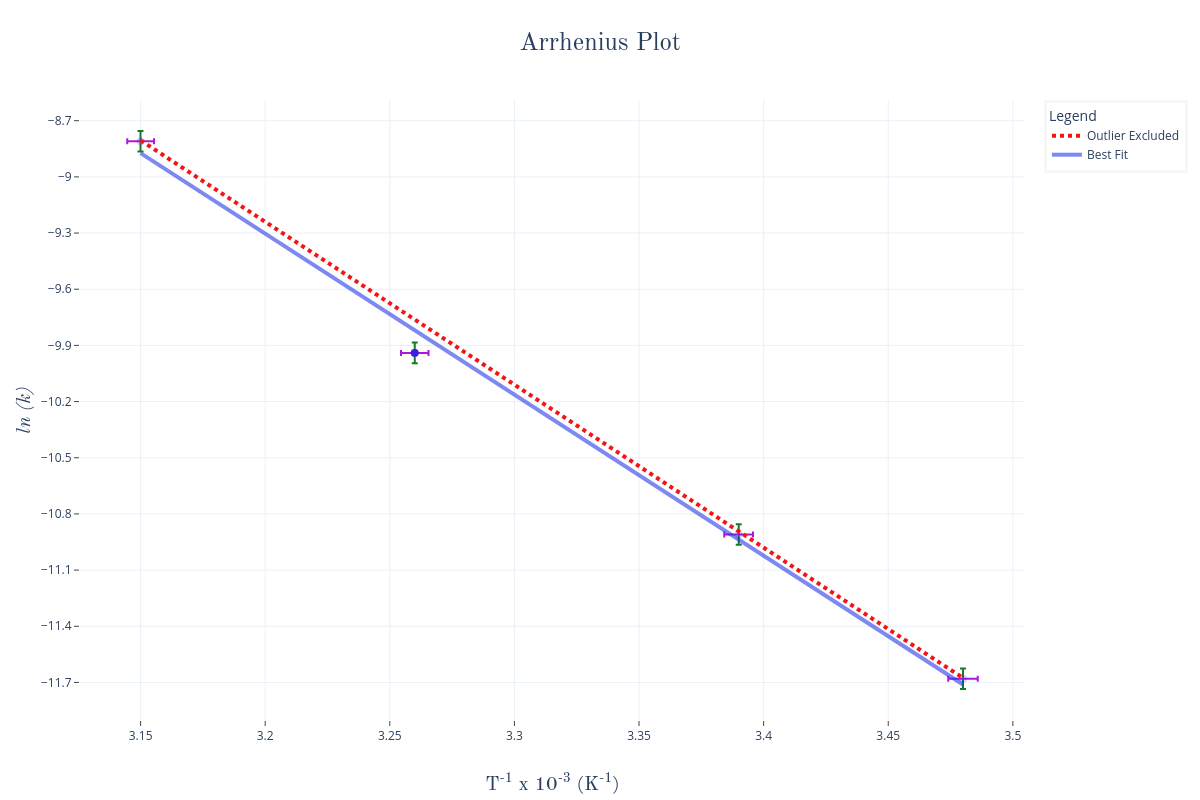
\includegraphics[width=1.0\textwidth]{fig/images/arrhenius.png}
    \caption{Arrhenius plot of $\ln{k}$ versus $\frac{1}{T}$ (scaled by $10^3$), including a best fit line for the general data and an improved trendline with the outlier removed.}
    \label{fig:arrhenius}
\end{figure}

\subsection{Analysis}
Overall, there do not appear to be any serious/obvious anomalies for all data collected in this experiment. The general trend line depicted in the linear regression of \cref{fig:arrhenius} is consistent with the scientific theory of the Arrhenius Equation and the linear relationship between the natural log of the rate constant and the inverse of the temperature of the reaction. The data collected for the trial at $\SI{294.8}{\kelvin}$ did appear to be an anomaly based on this statistical regression, however it was used to accurately determine the rate law for the overall stoichiometric reaction and its elimination did not result in a significantly larger correlation coefficient, indicating that it may not be as large of a structural deviation as initially thought. One possible explanation for this, however, may be that there were major fluctuations in room temperature at the time of the experiment, leading to a consistent change in proportions for all data calculated during thos trials. This explanation would account for the correct rate law being empirically derived from data at this temperature, and would also explain the reason for its status as an apparent outlier in the multi-temperature regression. The high $R^2$ value also suggests a strong statistical significance of the determined results, further providing support to the initial claims and lending credibility to the design and implementation of the experiment in its entirety. The uncertainties of the results were generally low for the majority of measurements, including those for temperature and volume, however the error for the final regression (and thus the activation energy) did become large due to a limited dataset size. This large error indicates systematic errors in the premise of the experiment, which will be further analyzed. 


\newpage

% !TEX root = ../chem_ia.tex
\section{Evaluation}

\subsection{Error Evaluation}

\subsubsection{Equipment}

\begin{table}[h!]
\centering

\begin{tabular}{|p{2.3cm}|p{1.5cm}|p{1.7cm}|p{1.5cm}|p{9.5cm}|}
\hline 
 Equipment & Absolute \newline Uncertainty & Smallest \newline Measurement & Percentage \newline Uncertainty & Significance/Improvement\\
 \hline
 Electric Timer (to determine time of reaction) & $\pm \SI{.05}{\second}$ & $\SI{37}{\second}$ & $.14\%$ & This is a very low percent error ($< .5\%$) and lends credibility to the results of the overall investigation. It is highly unlikely that human error with regards to the starting and stopping of the electric timer was a much larger contributor to overall issues with the final results, as opposed to the equipment itself. Thus, no material improvement is required for the purpose of time determinations. \\
 \hline
 $\SI{10}{\milli\liter}$ Graduated Cylinder (to measure out reactants) & $\pm \SI{.05}{\milli\liter}$ & $\SI{5}{\milli\liter}$ & $1\%$ & This is a moderate percent error, as it is still relatively low for the purpose and scope of the general investigation, but is quickly compounded. Because the volumes are used in a multitude of locations during the calculations (and there may be potential issues with the initial molarity), an improvement to the volumetric measuring process could drastically reduce overall experimental error. To achieve this beneficial result, a more precise measuring tool (such as a $\SI{1}{\milli\liter}$ syringe) could have been used.\\
 \hline

\end{tabular}
\caption{Equipment Error Evaluation}
\label{table:equipment_error_evaluation}
\end{table}

\subsubsection{Experimental Design}

\begin{table}[h!]
\centering

\begin{tabular}{|p{3cm}|p{7cm}|p{7cm}|}
\hline 
 Cause/Description & Impact on Results & Potential Alleviation\\
 \hline
 Limited Temperature Range (with a potential outlier) & Due to time and some feasibility constraints, only $4$ unique temperatures were chosen at which to run trials for the final activation energy experiment. These temperatures were relatively close magnitude-wise, indicating limited issues with intermediate temperature trends, however extreme temperatures were neglected on both ends of the spectrum. This could have caused serious drifts in the gradient calculation through the linear regression process. Additionally, $1$ of the $4$ temperatures appeared to provide outlier data, which was not thoroughly investigated nor confirmed. &  Obviously, more temperatures could have been used for testing purposes to assess whether extremely high or low temperatures cause serious deviations in the rate of the overall reaction. This would have also assisted in limiting the uncertainty with regards to the linear regression. It is, however, important to consider that at these extreme temperatures the reactant mixtures (containing water) could begin to boil or freeze, further introducing a confounding variable into the experiment.\\
 \hline
 Determination of completion of reaction (Random) & As iodine provides a strong color to the reactant mixture, a lack of color was relied for determining when the reaction had finished. This leads to potential variance with regards to the "specific" instance at which the reaction was truly finished and limits the consistency between trials. This issue is especially pertinent for quick trials (such as those at high temperatures), as the change is relatively rapid, and any hesitations or lack of sureness can have a serious impact on the final results. &  To remedy this, a spectrophotometer can be used to accurately measure wavelength absorbance of the reactant mixture during the duration of the reaction. This would ensure a consistent reading and limit human error with regards to the determination of completion. Due to issues with maintaining temperature equilibrium and the lack of resources, the device was not used for this investigation.\\
 \hline
 Inadequate Temperature Control (Random) & The impact of temperature on the rate constant inherently relies on maintaining a constant temperature for all reactants for the entirety of the reaction. However, because of the need for manual swirling while the reactants were in the water bath in addition to the open environment of the laboratory, it was difficult to accurately maintain the isolated temperature consistently. &  To ease the swirling process, an external magnetic stirring device could have been utilized to provide both more uniform mixing and limit the time spent outside the bath by the reactants. Ideally, a closed environment could be used to minimize external temperature fluctuations, however this was outside of the potential scope of this investigation. \\
 \hline
  Unaccounted change in concentrations of acid and acetone (Systematic) & The rate law determined for the reaction is $2nd$ order and depends on the concentration of $HCl$ and $Acetone$. To determine the rate, the assumption was made that the concentrations of these two reactants/catalysts remained constant, but there were obviously minor reductions for the concentration of both. This means that the simplification used to calculate the rate was not entirely accurate, as the rate did not stay even for the duration of the reaction. &  Some more complex mathematical techniques have been used in previous literature to attempt to better account for variations in the rate of the reaction over time, but they are largely out of the scope of this investigation. Overall, it has been found that ensuring $[HCl]$ and $[Acetone]$ significantly outweigh $[I_2]$ can minimize the error introduced by this issue, so it probably had limited impact on the final results.\\
 \hline

\end{tabular}
\caption{Experimental Design Error Evaluation}
\label{table:experimental_design_error_evaluation}
\end{table}

\subsubsection{Summary}

As demonstrated by \cref{table:equipment_error_evaluation}, there were limited equipment based errors for the majority of this experiment. Both of the primary tools used for measurement had uncertainties less than $1\%$, indicating that higher precision would not have drastically improved confidence or accuracy of the final results. It is important to note that the use of this equipment led to random error, as the determination of when to start and stop the timer was subject to the experimenter and varied between trials. \cref{table:experimental_design_error_evaluation} highlights both systematic and random errors associated with the actual design of the experiment itself. The lack of temperatures at which trials were conducted is the first major example of a systematic error, as this contributed to the final linear regression and drastically increased the uncertainty of the coefficients. Because the statistical approach of confidence intervals is inherently predicated on the degrees of freedom in the experiment (which approximately relates to the total data points), a lack of temperature ranges was a major inhibiter in producing more definite results. The lack of accountability in the change in concentration of the non-iodine reactants also provided another source of systematic error that could have been remedied to more accurately determine the rate of reaction. Prior literature has suggested that the concentrations of these reactants both undergo somewhat material fluctuations and can have large impacts on the rate of the otherwise slow iodination of acetone. The random errors of inadequate temperature control and a subjective mechanism for determining the completion of the reaction were also present, but would have required more complicated equipment and procedures to effectively control, which suggests that their alleviation is outside of the scope of this investigation. Overall, the investigation had a multitude of strengths and weaknesses in both the equipment utilized and the experimental procedure designed, which were partially discussed above and will be further analyzed in the subsequent comparison to documented scientific literature.

\subsection{Comparison to Scientific Literature}

The percent error of the result generated through this experiment ($\SI{71.01\pm14.27}{\kilo\joule\per\mole}$) and the accepted literature value from multiple papers ($\SI{86.60}{\kilo\joule\per\mole}$) was calculated to be $18\%$ in the results section. This error is larger than the $12\%$ uncertainty of the calculated result, indicating a serious systematic error in the methodology of this experiment. Therefore, it is worth comparing the procedure detailed throughout this paper and those employed by the various literature to analyze potential areas for improvement and justifications for the variation in the final result. The first approach was detailed by \textcite{other_literature_1} in which small quantities of the reaction mixture were drawn from the total reaction and passed through sodium bicarbonate and thiosulfate solution. The large concentrations of $HCl$ and $Acetone$ (as compared to $[I_2]$) was similar to that employed here, but the repeated usage of sodium bicarbonate and thiosulfate solution and the subsequent liberation of iodine was used to determine the rate of disappearance of iodine (or the overall rate of reaction of the iodination of acetone). This method allowed for more frequent assessments of the rate of the iodination reaction and provided more datapoints to ensure that the change in concentration of the non-iodine reactants was not affecting the rate. However, repeatedly opening the reactant solution to draw these samples out may have caused a similar issue to the presented investigation in which the temperature fluctuated. Overall, this procedure was unique in its lack of reliance on the light-absorbance of iodine solution, and was thus able to produce results with very limited uncertainty. In fact, the focus of the investigation was to minimize potential errors in the apparatus. Much of the difficulty in thoroughly comparing this investigation to \textcite{other_literature_1} is the large divide in equipment access and time constraints.

\textcite{reversiblity} also proposed a very similar experiment to \textcite{other_literature_1} by using titration techniques to repeatedly determine the rate of removal of $I_2$ from the reactant mixture, however they incorporated a buffer solution via the addition of potassium iodate to maintain the relative pH value of the overall solution. This helped introduce the discovery that this reaction between iodine and acetone is highly reversible in strongly acid solutions, which was initially discussed by \textcite{reversibility_find}. It is important to recognize that $HCl$ simply behaves as a catalyst in this reaction, it is not an active reactant, and thus it lowers the activation energy of both the forward and backward reaction. Both of the reactions are exceedingly slow in the absence of a catalyst (especially as compared to the general halogenation of many organic compounds), however the introduction of an acid catalyst allows for a more feasible reaction in both directions. At moderately acidic pH values for the reaction mixture, this allows for an eventual equilibrium shifted distinctively to the right. However, for more concentrated acidic solutions ($>\SI{.05}{\molar}$), the backwards reaction becomes more feasible, shifting the equilibrium towards the left and preventing the complete halogenation of the reaction. This result is particularly influential for the investigation presented here, as the production of reactants in the reverse reaction would have artifically inflated the total duration of the reaction and produced incorrect calculations for the rate of consumption of $I_2$ solution. The introducation of buffer solutions, as used by \textcite{reversiblity}, can prevent large fluctuations in the pH of the solution mixture, especially after the intermediate production of enols (which are slightly acidic themselves). This result also indicates an "optimal" concentration of $H^+$ ions at which the equilibrium constant is maximum and the time required for equilibrium to be reached is minimum, which would be worth further investigation via the use of various acidic concentrations.

A more traditional approach to the study of this reaction is also described by \textcite{main_literature}, where the absorbance of iodine and the change in absorbance of the reaction mixture is measured with the help of a spectrophotometer to determine the rate of the reaction at various points. This procedure was able to generate highly consistent (and accurate) results with limited trials through the use of a differential method for activation energy calculations. Although the mathematical premise of the investigation falls outside of the scope of this research, the introduction of absorbance data could facilitate an easier mechanism for calculating the activation energy and provide a more relevant baseline for comparison with the linear regression. The use of a spectrophotomer does require constant transfer of small quantities of the reaction mixture from the temperature-stable vessel to the external machine. To minimize heat loss to the surroundings, \textcite{main_literature} were able to use thermostatted pipettes which would most likely not have been feasible for this experiment.

\subsection{Extensions}

Many of the potential methodological extensions/improvements to this investigation were discussed in the comparison to external literature, however, there are other relevant extensions that could provide important information for industrial and theoretical purposes. Com{}paring various acidic catalysts and alternative halogens for this type of reaction could assist in determining optimal techniques for mass production of enols and improving the ability to rationalize the differences in proposed mechanisms for enolization in acidic-solutions. It would also be intriguing to compare this investigation to the same reaction with a basic catalyst. These experiments could provide an ability to investigate different potential products and the direct impact of the pH of the reactant mixture on the rate and mechanism of the general iodination of acetone~\parencite{base_catalyst}.

% !TEX root = ../math_ia.tex
\section{Conclusion}

This investigation attempted to explore the fascinating world of physical moment of inertias by highlighting unique methods of mathematical derivations. Using the basic definition of moment of inertia presented at the beginning of the paper, it was trivial to determine the value for simple point masses or hollow shapes. Basic integration, elemental mass areas, and vectorized/matrix-oriented approaches were all utilized for further calculations for more complex bodies, culminating in the final extension which provides a result to calculate the moment of inertia for any 3-D body about any axis, obviously an extremely powerful and streamlined tool for physics-based math. 

Scientists and mathematicians continue to work on deriving methods for these types of calculations for highly irregular bodies, such as those found in nature, and on optimizing rotational inertia to improve engineering-based applications in the real-world. Advancements in multivariable calculus and matrix factorization have already allowed for more complex implementations of the extension formula, and the results emphasize the importance of mathematics in the physical realm. Obviously, a logical step for further research and the verification of the results presented here would be a real-world study of the movement of these uniquely shaped bodies. By providing a known angular velocity, the theoretical results could be confirmed or rejected, and potentially allow for more nuanced discoveries about internal and environmental factors which affect the rotational movement of rigid bodies. It is obviously imperative to remember that these are all purely abstract derivations and thus simply provide our approximate and ideal guess as to the moments for the bodies discussed previously. The deliberate mathematical approach is both a strength and weakness as it limits external factors and avoids the issue of confounding and uncontrollable factors which may plague a practical laboratory experiment, but also may struggle to account for individual discrepancies or allow for a more nuanced debate surrounding external factors that contribute to the findings. Overall, the work still facilitates a general understanding of moment of inertia for progressively more complex bodies while highlighting the future of the field and discussing new techniques which can improve the generalizablity of these important results.

\printbibliography
\end{document}{}
